\chapter{Présentation du Projet}

\section{Objectif}

L’objectif principal de ce projet est de concevoir et de développer une application mobile météo permettant aux utilisateurs d’accéder facilement et rapidement aux informations météorologiques pertinentes, où qu’ils se trouvent. Cette application vise à être un outil pratique, fiable et convivial, adapté au grand public.

\noindent Les objectifs du projet sont les suivants :

\begin{itemize}
    \item Fournir des prévisions météorologiques précises et régulièrement mises à jour grâce à une API dédiée.
    
    \item Offrir une expérience utilisateur simple et intuitive afin de garantir un accès rapide aux informations essentielles telles que la température, les précipitations, l’humidité et la vitesse du vent.
    
    \item Permettre la géolocalisation automatique afin d’afficher la météo actuelle en fonction de la position de l’utilisateur.
    
    \item Inclure une fonctionnalité de recherche par ville permettant de consulter la météo d’autres localités.
    
    \item Assurer une compatibilité multi-plateforme (Android et iOS) afin de toucher un maximum d’utilisateurs.
    
    \item Mettre en place un système de notifications météo (facultatif) pour alerter l’utilisateur en cas de conditions météorologiques particulières (orages, canicule, fortes pluies, etc.).
    
    \item Prévoir la possibilité d’ajouter des fonctionnalités futures, telles que les alertes météo avancées ou l’affichage de cartes interactives.
\end{itemize}


\section{Justification et caractère innovant du projet}

Aujourd’hui, les informations météorologiques sont souvent présentées sous forme de bulletins ou de pages statiques sur des sites web. Même si ces informations restent utiles, elles ne permettent pas toujours d’explorer facilement les données ou d’observer leur évolution dans le temps.\\

\noindent Le projet URGmetEO propose une approche plus interactive. En effet, la plateforme permet non seulement de consulter les données météorologiques, mais aussi de les visualiser à l’aide de graphiques et de cartes. Cette représentation rend les informations plus claires et facilite leur interprétation. Par ailleurs, le projet intègre également un dispositif IoT basé sur un microcontrôleur ESP-32D qui permet de signaler certaines conditions météorologiques à l’aide d’indicateurs lumineux. Cette combinaison entre collecte de données, visualisation et dispositif matériel constitue un aspect innovant du projet.

 \section{Les risques}
 Dans tout projet informatique, plusieurs facteurs peuvent influencer la bonne réalisation du système. Dans le cadre du projet URGmetEO, certains risques ont été identifiés. Ces risques peuvent être classés en trois catégories principales : les risques fonctionnels, les risques techniques et les risques économiques.
 
 \subsection{Risques sur le plan fonctionnel}

Les risques fonctionnels concernent principalement le bon fonctionnement de l’application ainsi que la fiabilité des informations météorologiques fournies aux utilisateurs.

\paragraph{Données météorologiques inexactes ou retardées}

Tout d’abord, l’application URGmetEO repose sur des données météorologiques provenant de stations de mesure. Si ces données sont inexactes, incomplètes ou mises à jour avec retard, les informations affichées dans l’application peuvent devenir incorrectes. Cela peut entraîner une mauvaise interprétation des conditions météorologiques, l’émission d’alertes inappropriées ou encore une perte de confiance des utilisateurs. Il est donc important de s’assurer de la fiabilité de la source des données et de vérifier régulièrement la validité des informations reçues.

\paragraph{Problèmes de localisation}

Par ailleurs, l’application utilise la géolocalisation du téléphone afin de fournir des informations météorologiques adaptées à la position de l’utilisateur. Toutefois, certaines difficultés peuvent apparaître, notamment en raison d’une imprécision du GPS, du refus de l’utilisateur d’autoriser l’accès à la localisation ou encore de difficultés à déterminer la position dans certaines zones. Dans ces situations, l’application peut rencontrer des difficultés à afficher les informations météorologiques correspondant à la localisation réelle de l’utilisateur.

\subsubsection{Risques sur le plan technique}

Les risques techniques concernent principalement les technologies utilisées pour développer et faire fonctionner le système URGmetEO. Ils peuvent affecter la disponibilité des données, la communication entre les différents composants du système ou encore le bon fonctionnement de l’application mobile.

\paragraph{Problèmes de connexion Internet}

Tout d’abord, le fonctionnement de l’application dépend fortement de la connexion Internet. Une connexion instable ou une absence de réseau peut empêcher la récupération des données météorologiques, la mise à jour des informations affichées dans l’application ou encore la communication avec les services distants. Dans ce cas, l’utilisateur pourrait ne pas recevoir les informations météorologiques au moment opportun.

\paragraph{Défaillance de l’API météo}

Ensuite, l’application s’appuie sur une API météorologique externe pour obtenir les prévisions. Si cette API devient indisponible, subit des modifications techniques ou atteint une limite d’utilisation, certaines fonctionnalités de l’application pourraient être affectées. Cette dépendance à un service externe représente donc un risque pour la continuité du système.

\paragraph{Compatibilité des appareils mobiles}

Par ailleurs, l’application mobile URGmetEO est développée avec React Native et l’environnement Expo afin d’être compatible avec plusieurs plateformes mobiles. Toutefois, des problèmes de compatibilité peuvent apparaître selon les appareils utilisés. Ces difficultés peuvent être liées aux différences entre les versions d’Android et d’iOS, à la gestion des autorisations système (comme l’accès à la localisation GPS) ou encore aux limitations matérielles de certains appareils. Ces facteurs peuvent entraîner des variations de performance ou des dysfonctionnements de certaines fonctionnalités. Afin de limiter ces risques, il est nécessaire de tester l’application sur plusieurs appareils et différentes versions de systèmes d’exploitation.

\paragraph{Communication avec le module IoT ESP-32D}

Enfin, le projet URGmetEO intègre un dispositif IoT basé sur un microcontrôleur ESP-32D permettant de signaler les conditions météorologiques à l’aide de LEDs. Toutefois, des difficultés de communication peuvent apparaître entre l’application et ce module, notamment en raison de problèmes de configuration du réseau Wi-Fi, d’interruptions du réseau local ou d’erreurs dans les requêtes HTTP. Dans ces situations, les indicateurs lumineux pourraient ne pas refléter correctement les conditions météorologiques détectées.
\subsection{Risques économiques}

Les risques économiques concernent les ressources financières nécessaires au déploiement, à l’exploitation et à la maintenance du système.

\subsubsection{Coût d’infrastructure et de déploiement}

Dans le cadre du projet URGmetEO, les données météorologiques ne sont pas générées directement par l’application. Elles proviennent d’un serveur distant mis à disposition par l’organisme URGEO, lequel collecte les informations en temps réel à partir de plusieurs stations météorologiques installées dans différentes régions du pays.\\

\noindent L’application mobile et le backend du projet doivent donc interagir avec cette infrastructure afin de récupérer et d’exploiter ces données.\\

\noident Cependant, la mise en production du système nécessite certaines ressources techniques pouvant engendrer des coûts, notamment :


\begin{itemize}
\item l’hébergement du backend (API) permettant de traiter les requêtes provenant de l’application mobile ;
\item le déploiement de l’application mobile sur les plateformes de distribution telles que le Play Store et l’App Store ;
\item les services de réseau et de sécurité nécessaires pour assurer la communication entre l’application, le backend et le serveur de données météorologiques ;
\item la gestion de l’infrastructure logicielle utilisée pour garantir la disponibilité et la fiabilité du système.
\end{itemize}


\subsubsection{Maintenance de l’infrastructure}

Une fois le système déployé, des opérations de maintenance sont nécessaires afin d’assurer son bon fonctionnement dans le temps. Cette maintenance peut inclure :

\begin{itemize}
\item la mise à jour de l’application mobile ;
\item l’amélioration des performances du backend ;
\item l’adaptation du système aux évolutions du serveur de données météorologiques fourni par URGEO ;
\item la correction des éventuelles anomalies détectées après le déploiement.
\end{itemize}


 \section{État de l’art}

 \subsection{ Situation actuelle en Haïti}
 En Haïti, l’organisme principalement responsable de la surveillance météorologique est l’Unité Hydrométéorologique d’Haïti (UHM). Cette institution met à disposition du public différentes informations climatiques à travers son site web officiel : \textit{http://www.meteo-haiti.gouv.ht}.

\noindent Le site propose principalement des bulletins météorologiques, des prévisions climatiques ainsi que des images satellites couvrant la région caribéenne. Les informations diffusées concernent notamment la température, les précipitations, la vitesse du vent et les conditions atmosphériques générales.\\

\noindent Toutefois, les données disponibles sont généralement présentées sous forme de bulletins ou de cartes statiques. Il est donc difficile pour les utilisateurs d’explorer ces informations de manière interactive ou d’effectuer des analyses basées sur des données historiques. Dans ce contexte, le développement d’une plateforme permettant la collecte, le stockage et la visualisation dynamique des données météorologiques pourrait faciliter l’accès et l’exploitation de ces informations.

\begin{figure}[H]
    \centering
   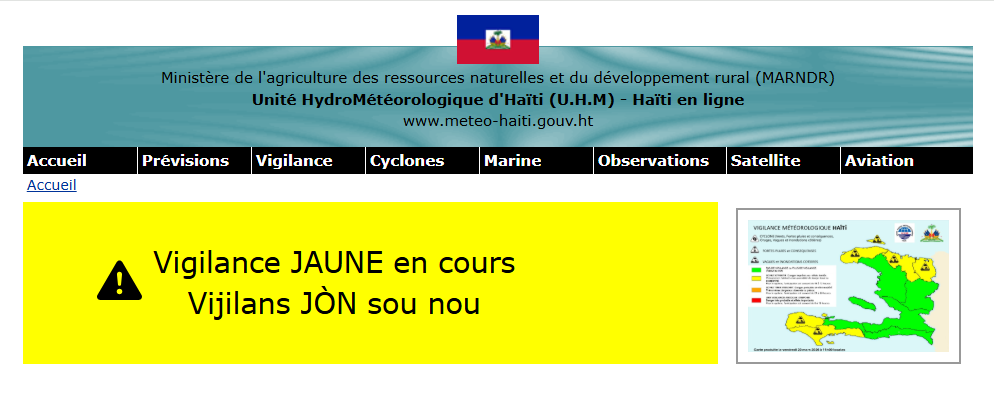
\includegraphics[width=1
   \textwidth]{UHM.png}
    \caption{Page d'accueil de www.meteo-haiti.gouv.ht}
    \label{fig:placeholder}
\end{figure}
 \newpage
 \subsection{Technologies de visualisation des données météorologiques dans le monde}
 
 \subsubsection{Meteostat}
 Meteostat est une plateforme mondiale qui fournit des données météorologiques historiques et en temps réel provenant de nombreuses stations réparties dans le monde. Elle met à disposition différentes informations climatiques telles que la température, les précipitations, la vitesse du vent ou encore l’humidité. Les utilisateurs peuvent accéder à ces données à travers une interface web ou via une API permettant leur intégration dans différentes applications.

\begin{figure}[H]
    \centering
   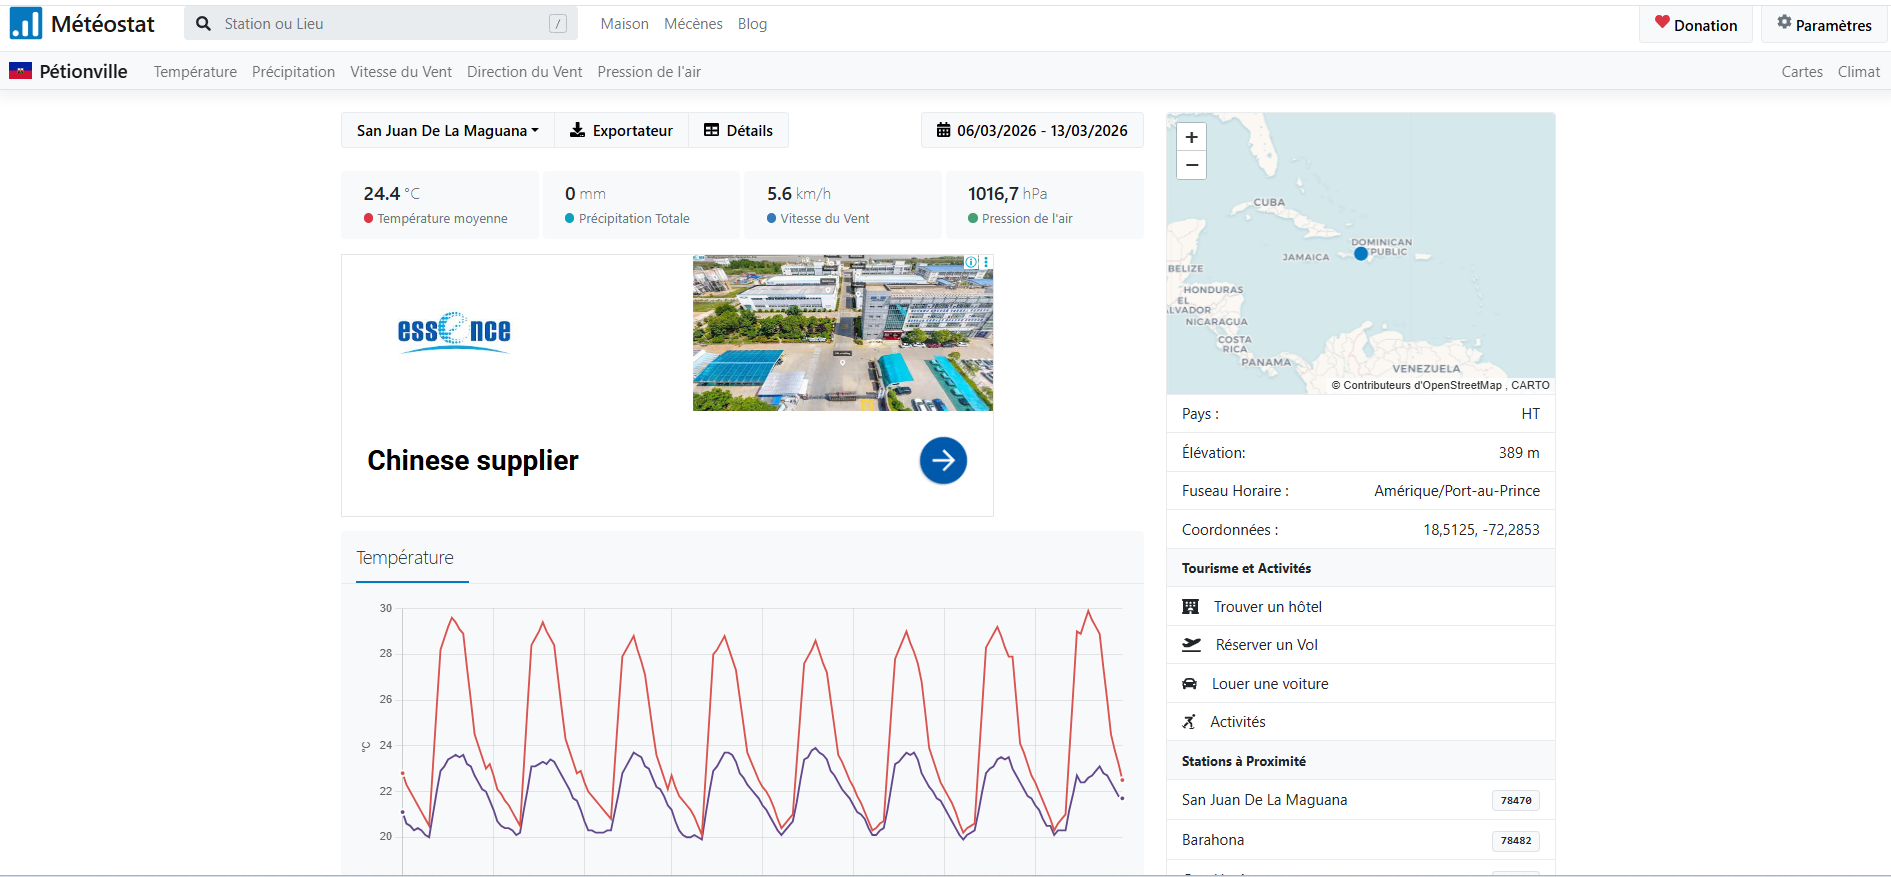
\includegraphics[width=1\textwidth]{Meteostat.png}
    \caption{Page d'accueil de Méteostat}
    \label{fig:placeholder}
\end{figure}


 \subsubsection{Windy}
 Windy est une plateforme de visualisation météorologique interactive qui permet d’explorer les conditions météorologiques à l’aide de cartes dynamiques. L’application affiche différentes variables telles que le vent, la température ou les précipitations, et permet d’observer leur évolution dans le temps grâce à des outils d’animation et de visualisation.

\begin{figure}[H]
    \centering
   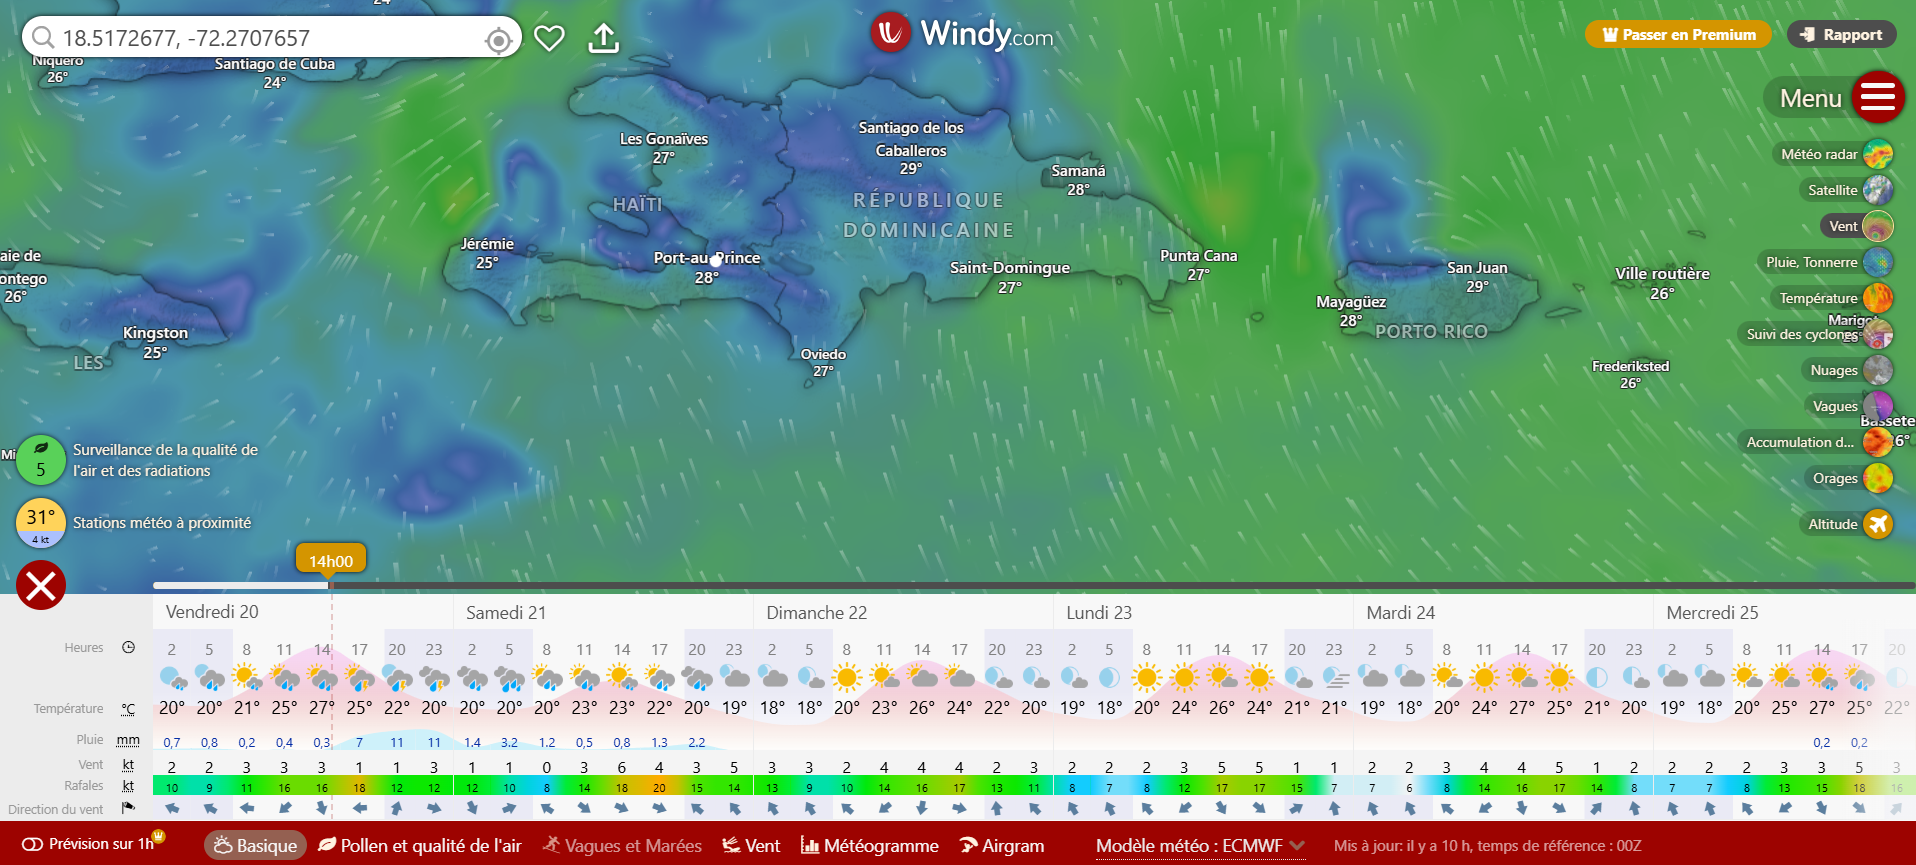
\includegraphics[width=1\textwidth]{Windy.png}
    \caption{Page d'accueil de Windy}
    \label{fig:placeholder}
\end{figure}
\newpage
 \subsubsection{Meteoblue}
 Meteoblue est un service météorologique international qui propose des prévisions et des données climatiques pour différentes régions du monde. La plateforme s’appuie sur des modèles de prévision atmosphérique combinés à des données provenant de stations météorologiques afin de fournir des informations détaillées sous forme de graphiques et de cartes.

 \begin{figure}[H]
    \centering
   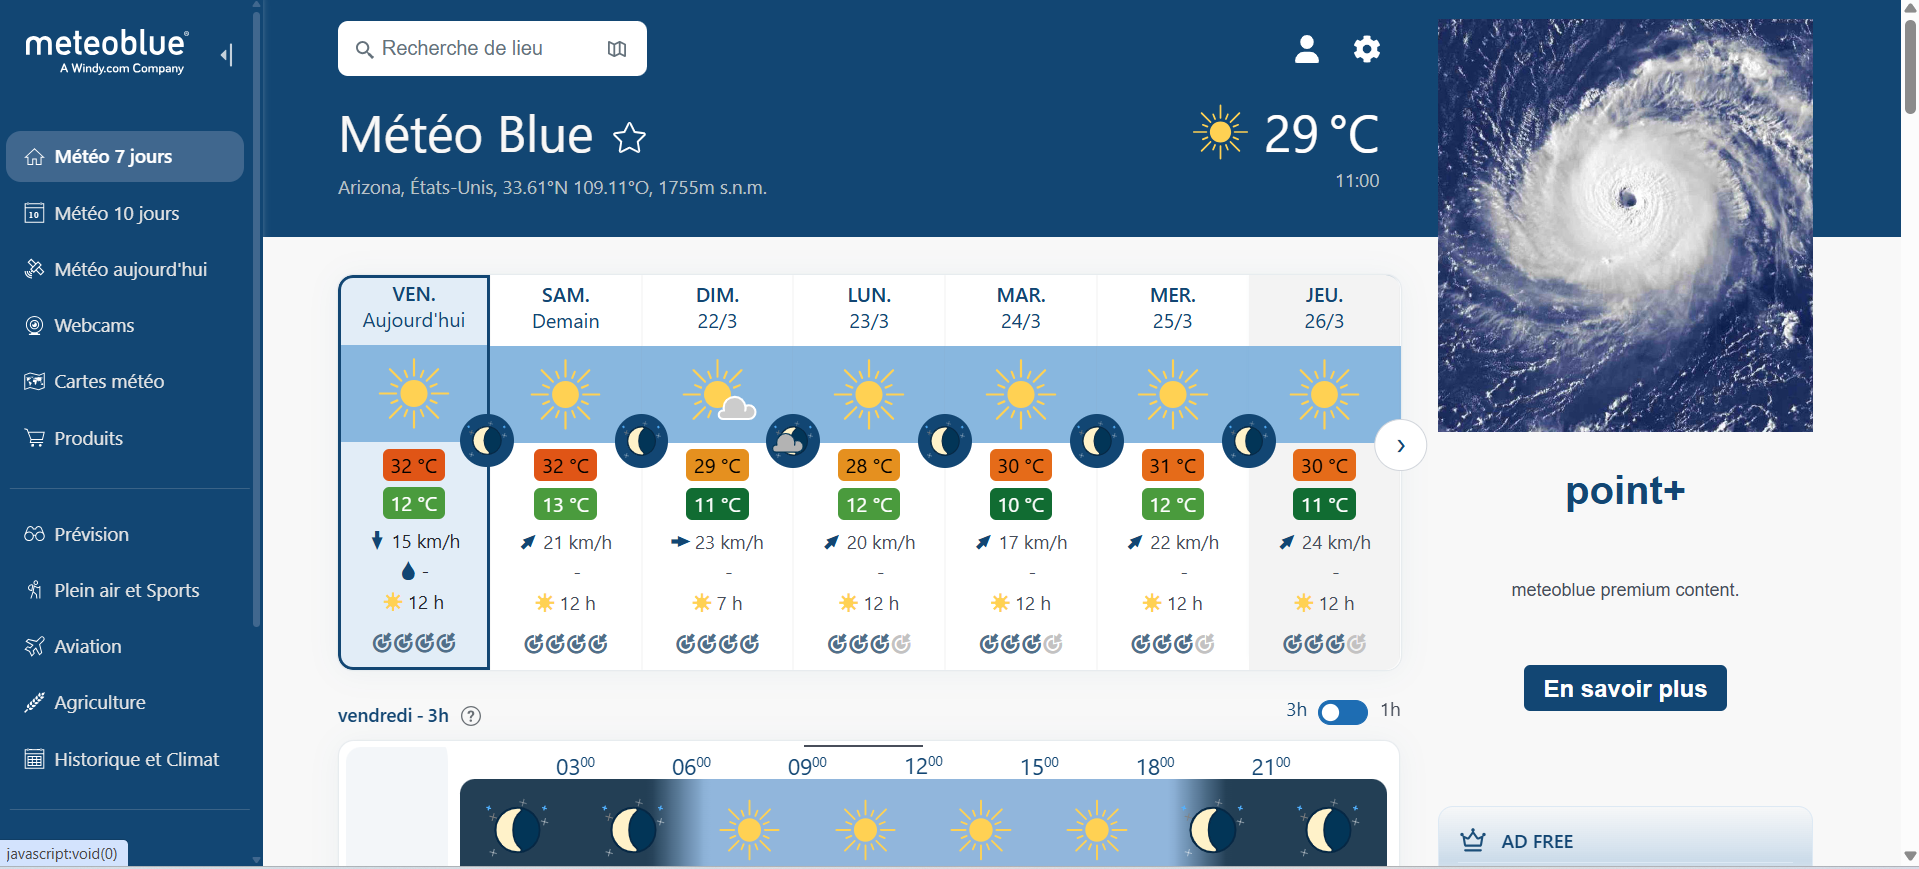
\includegraphics[width=1\textwidth]{Meteoblue.png}
    \caption{Page d'accueil de Meteoblue}
    \label{fig:placeholder}
\end{figure}

\subsubsection{OpenWeatherMap}
 OpenWeatherMap est une plateforme populaire qui fournit des données météorologiques à travers des services web et des interfaces de programmation (API). Elle permet aux développeurs d’intégrer facilement des informations telles que la température, la pression atmosphérique, l’humidité ou les prévisions météorologiques dans différentes applications.\\

 \begin{figure}[H]
    \centering
   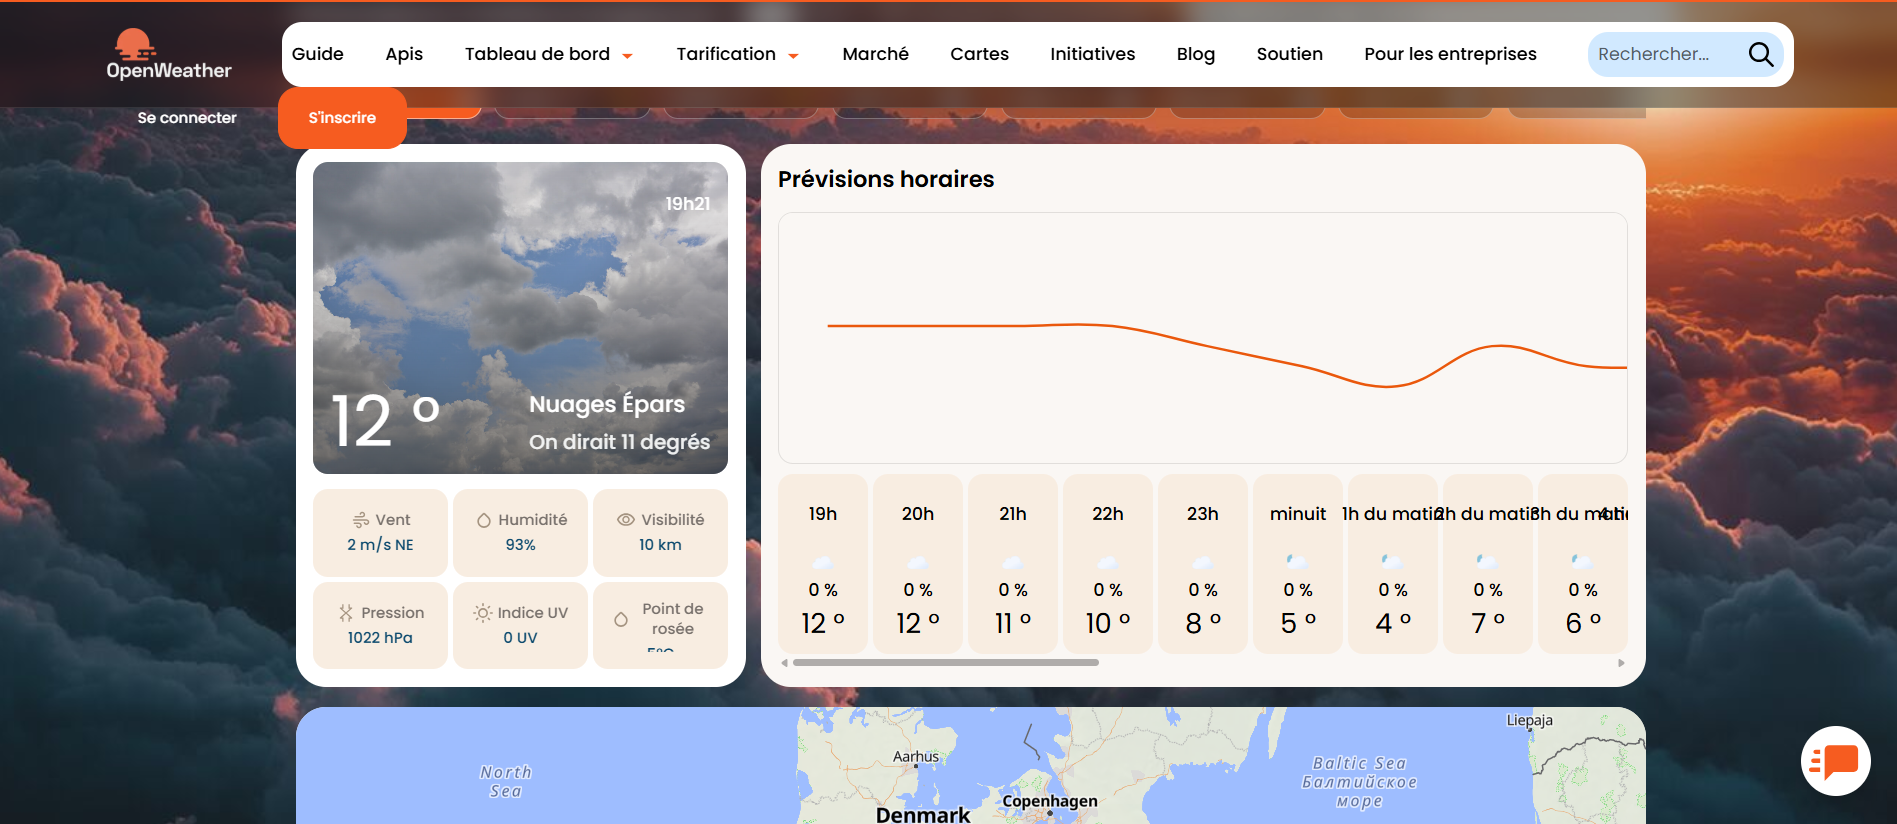
\includegraphics[width=1\textwidth]{Openweathmap.png}
    \caption{Page d'accueil d'OpenWeatherMap}
    \label{fig:placeholder}
\end{figure}

 \subsection{Limites des solutions existantes}

Malgré la disponibilité de plusieurs plateformes météorologiques, l’accès aux données reste souvent limité à des bulletins ou à des informations statiques. Dans de nombreux cas, les utilisateurs ne disposent pas d’outils permettant d’explorer les données de manière interactive ou d’observer facilement leur évolution dans le temps.

\noident De plus, ces solutions se concentrent généralement sur la simple diffusion d’informations météorologiques. Elles offrent peu de possibilités de visualisation dynamique ou d’analyse des tendances climatiques, ce qui peut rendre l’interprétation des données plus difficile pour les utilisateurs.

\noident Enfin, les mécanismes d’alerte et les options de personnalisation sont parfois limités. Les utilisateurs ne peuvent pas toujours adapter l’affichage des informations selon leurs besoins ou recevoir des notifications adaptées à certaines conditions météorologiques.


\subsection{Contribution et valeur ajoutée de la solution URGmetEO}

Dans ce contexte, la solution URGmetEO propose une approche plus interactive pour l’exploitation des données météorologiques. Tout d’abord, la plateforme permet de centraliser les informations climatiques et d’y accéder en temps réel à travers une interface simple et interactive. Les utilisateurs peuvent ainsi consulter facilement les conditions météorologiques actuelles depuis une application mobile, quel que soit leur emplacement.

Ensuite, URGmetEO ne se limite pas à l’affichage de données brutes. Le système intègre des outils de visualisation tels que des graphiques dynamiques et des cartes géographiques, facilitant ainsi l’analyse des tendances climatiques et la compréhension de l’évolution des phénomènes météorologiques.

Par ailleurs, la plateforme propose un système d’alertes météorologiques basé sur des seuils prédéfinis. Ce mécanisme permet d’informer rapidement les utilisateurs en cas de conditions météorologiques particulières ou potentiellement dangereuses.

Enfin, la solution offre également des possibilités de personnalisation de l’interface. Les utilisateurs peuvent adapter l’affichage des informations selon leurs préférences, notamment en choisissant les unités de mesure ou les paramètres météorologiques qu’ils souhaitent consulter.


 \section{Analyse des besoins du projet}
 
